\documentclass[journal,12pt,twocolumn]{IEEEtran}
\usepackage{amsthm}
\allowbreak
\usepackage{setspace}
\usepackage{gensymb}
\singlespacing
\usepackage[cmex10]{amsmath}
\usepackage{caption}
\usepackage{amsthm}
\usepackage{float}

\DeclareUnicodeCharacter{2212}{-}
\usepackage{tikz}
\usepackage{pgfplots}

\usepackage{mathrsfs}
\usepackage{txfonts}
\usepackage{stfloats}
\usepackage{bm}
\usepackage{cite}
\usepackage{cases}
\usepackage{subfig}

\usepackage{longtable}
\usepackage{multirow}

\usepackage{enumitem}
\usepackage{mathtools}
\usepackage{steinmetz}
\usepackage{tikz}
\usepackage{circuitikz}
\usepackage{verbatim}
\usepackage{tfrupee}
\usepackage[breaklinks=true]{hyperref}
\usepackage{graphicx}
\usepackage{tkz-euclide}
\graphicspath{ {./images/} }
\usetikzlibrary{calc,math}
\usepackage{listings}
    \usepackage{color}                                            %%
    \usepackage{array}                                            %%
    \usepackage{longtable}                                        %%
    \usepackage{calc}                                             %%
    \usepackage{multirow}                                         %%
    \usepackage{hhline}                                           %%
    \usepackage{ifthen}                                           %%
    \usepackage{lscape}     
\usepackage{multicol}
\usepackage{chngcntr}

\DeclareMathOperator*{\Res}{Res}

\renewcommand\thesection{\arabic{section}}
\renewcommand\thesubsection{\thesection.\arabic{subsection}}
\renewcommand\thesubsubsection{\thesubsection.\arabic{subsubsection}}

\renewcommand\thesectiondis{\arabic{section}}
\renewcommand\thesubsectiondis{\thesectiondis.\arabic{subsection}}
\renewcommand\thesubsubsectiondis{\thesubsectiondis.\arabic{subsubsection}}


\hyphenation{op-tical net-works semi-conduc-tor}
\def\inputGnumericTable{}                                 %%

\lstset{
%language=C,
frame=single, 
breaklines=true,
columns=fullflexible
}
\begin{document}


\newtheorem{theorem}{Theorem}[section]
\newtheorem{problem}{Problem}
\newtheorem{proposition}{Proposition}[section]
\newtheorem{lemma}{Lemma}[section]
\newtheorem{corollary}[theorem]{Corollary}
\newtheorem{example}{Example}[section]
\newtheorem{definition}[problem]{Definition}

\newcommand{\BEQA}{\begin{eqnarray}}
\newcommand{\EEQA}{\end{eqnarray}}
\newcommand{\define}{\stackrel{\triangle}{=}}
\bibliographystyle{IEEEtran}
\raggedbottom
\setlength{\parindent}{0pt}
\providecommand{\mbf}{\mathbf}
\providecommand{\pr}[1]{\ensuremath{\Pr\left(#1\right)}}
\providecommand{\qfunc}[1]{\ensuremath{Q\left(#1\right)}}
\providecommand{\sbrak}[1]{\ensuremath{{}\left[#1\right]}}
\providecommand{\lsbrak}[1]{\ensuremath{{}\left[#1\right.}}
\providecommand{\rsbrak}[1]{\ensuremath{{}\left.#1\right]}}
\providecommand{\brak}[1]{\ensuremath{\left(#1\right)}}
\providecommand{\lbrak}[1]{\ensuremath{\left(#1\right.}}
\providecommand{\rbrak}[1]{\ensuremath{\left.#1\right)}}
\providecommand{\cbrak}[1]{\ensuremath{\left\{#1\right\}}}
\providecommand{\lcbrak}[1]{\ensuremath{\left\{#1\right.}}
\providecommand{\rcbrak}[1]{\ensuremath{\left.#1\right\}}}
\theoremstyle{remark}
\newtheorem{rem}{Remark}
\newcommand{\sgn}{\mathop{\mathrm{sgn}}}
\providecommand{\abs}[1]{$\left\vert#1\right\vert$}
\providecommand{\res}[1]{\Res\displaylimits_{#1}} 
\providecommand{\norm}[1]{$\left\lVert#1\right\rVert$}
%\providecommand{\norm}[1]{\lVert#1\rVert}
\providecommand{\mtx}[1]{\mathbf{#1}}
\providecommand{\mean}[1]{E$\left[ #1 \right]$}
\providecommand{\fourier}{\overset{\mathcal{F}}{ \rightleftharpoons}}
%\providecommand{\hilbert}{\overset{\mathcal{H}}{ \rightleftharpoons}}
\providecommand{\system}{\overset{\mathcal{H}}{ \longleftrightarrow}}
	%\newcommand{\solution}[2]{\textbf{Solution:}{#1}}
\newcommand{\solution}{\noindent \textbf{Solution: }}
\newcommand{\cosec}{\,\text{cosec}\,}
\providecommand{\dec}[2]{\ensuremath{\overset{#1}{\underset{#2}{\gtrless}}}}
\newcommand{\myvec}[1]{\ensuremath{\begin{pmatrix}#1\end{pmatrix}}}
\newcommand{\mydet}[1]{\ensuremath{\begin{vmatrix}#1\end{vmatrix}}}
\numberwithin{equation}{subsection}
\makeatletter
\@addtoreset{figure}{problem}
\makeatother
\let\StandardTheFigure\thefigure
\let\vec\mathbf
\renewcommand{\thefigure}{\theproblem}
\def\putbox#1#2#3{\makebox[0in][l]{\makebox[#1][l]{}\raisebox{\baselineskip}[0in][0in]{\raisebox{#2}[0in][0in]{#3}}}}
     \def\rightbox#1{\makebox[0in][r]{#1}}
     \def\centbox#1{\makebox[0in]{#1}}
     \def\topbox#1{\raisebox{-\baselineskip}[0in][0in]{#1}}
     \def\midbox#1{\raisebox{-0.5\baselineskip}[0in][0in]{#1}}
\vspace{3cm}
\title{AI1103: Assignment 2}
\author{Damaragidda Bharadwaja Rao - CS20BTECH11012}
\maketitle
\newpage
\bigskip
\renewcommand{\thefigure}{\theenumi}
\renewcommand{\thetable}{\theenumi}
Download all python codes from 
\begin{lstlisting}
https://github.com/Bharadwaja-rao-D/AI1103/blob/main/assignment2/assignment2.py
\end{lstlisting}
%
and latex-tikz codes from 
%
\begin{lstlisting}
https://github.com/Bharadwaja-rao-D/AI1103/blob/main/assignment2/assignment2.tex
\end{lstlisting}
\section*{Problem GATE-EC-Q40: }
A digital communication system uses a
repetition code for channel
encoding/decoding. During transmission, each
bit is repeated three times(0 is transmitted as
000, and 1 is transmitted as 111). It is
assumed that the source puts out symbols
independently and with equal probability. The
decoder operates as follows: In a block of three
received bits, if the number of zeros exceeds the
number of ones, the decoder decides in favour of
a 0, and if the number of ones exceeds the
number of zeros, the decoder decides in favour
of a 1. Assuming a binary symmetric channel
with crossover probability p = 0.1, the average
probability of error is
\section*{Solution:}
Let Y be the bit sent by the sender and X be the number of 1's received by the receiver and p = 0.1 is the crossover probability
\subsection*{Case 1: Y = 0}

\begin{align}
    \Pr(X = i) &= \binom{n}{i}\times p^i\times (1-p)^{n-i}\\
\Pr(X = 0) &= \binom{3}{0}\times p^0\times (1-p)^{3}\\
\Pr(X = 1) &= \binom{3}{1}\times p^1\times (1-p)^{2}\\
\Pr(X = 2) &= \binom{3}{2}\times p^2\times (1-p)^{1}\\
\Pr(X = 3) &= \binom{3}{3}\times p^3\times (1-p)^{0}
\end{align}
When $X \geq 2 $ the receiver interprets it as 1, which is an error. And by Total Probability theorem we have\\
\begin{align}
P_1 = \frac{P(X = 2) + P(X = 3)}{\sum_{i=0}^3P(X = i)}
\end{align}
where $P_1$ is the probability of error when Y = 0
\subsection*{Case 2: Y = 1}
\begin{align}
\Pr(X = i) &= \binom{n}{i}\times p^{n-i}\times (1-p)^i\\
\Pr(X = 0) &= \binom{3}{0}\times p^3\times (1-p)^{0}\\
\Pr(X = 1) &= \binom{3}{1}\times p^2\times (1-p)^{1}\\
\Pr(X = 2) &= \binom{3}{2}\times p^1\times (1-p)^{2}\\
\Pr(X = 3) &= \binom{3}{3}\times p^0\times (1-p)^{3}
\end{align}
When $X \leq 1 $ the receiver interprets it as 0, which is an error. And by Total Probability theorem we have
\begin{align}
P_2 = \frac{\Pr(X = 0) + \Pr(X = 1)}{\sum_{i=0}^3\Pr(X = i)}
\end{align}
where $P_2$ is the probability of error when Y = 1
\begin{multline}
\sum_{i=0}^3\Pr(X = i) = 1\times 0.9^3 + 3\times 0.1\times 0.9^2 \\
+ 3\times 0.1^2 \times 0.9 + 1\times 0.1^3 = 1
\end{multline}
\begin{align}
P_1 &= 0.028\\
P_2 &= 0.028
\end{align}
The average probability is 
\begin{multline}
P_{avg} = \Pr(Y = 0)\times P_1 +\Pr(Y = 1)\times P_2\\ = 0.028 \end{multline}
\begin{table}[H]
\centering
\resizebox{\columnwidth}{!cm}{
\begin{tabular}{|c|c|c|c|c|c|}
\hline
     &X&0&1&2&3  \\
     \hline
     Y=0&\Pr(X)&0.729&0.243&0.027&0.001\\
     \hline
     Y=1&\Pr(X)&0.001&0.027&0.243&0.729\\
     \hline
\end{tabular}
}
\caption{Probability of number of 1's recieved  }
\label{table:1}
\end{table}
\begin{figure}[htp]
    \centering
    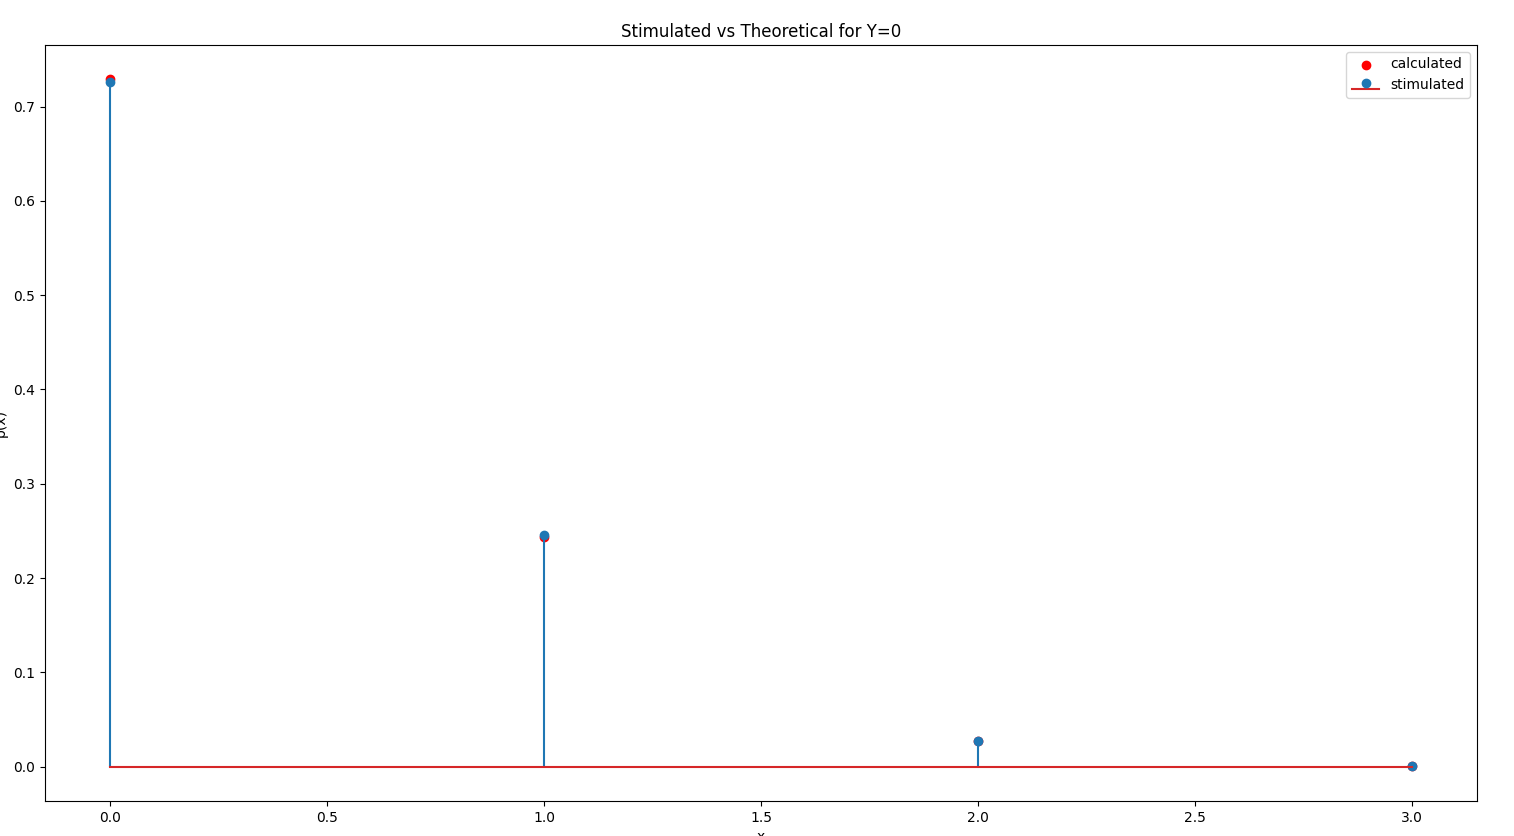
\includegraphics[width=8cm]{assignment2_plot1}
    \caption{Plot when Y = 0}
    \label{fig:1}
\end{figure}
\begin{figure}[htp]
    \centering
    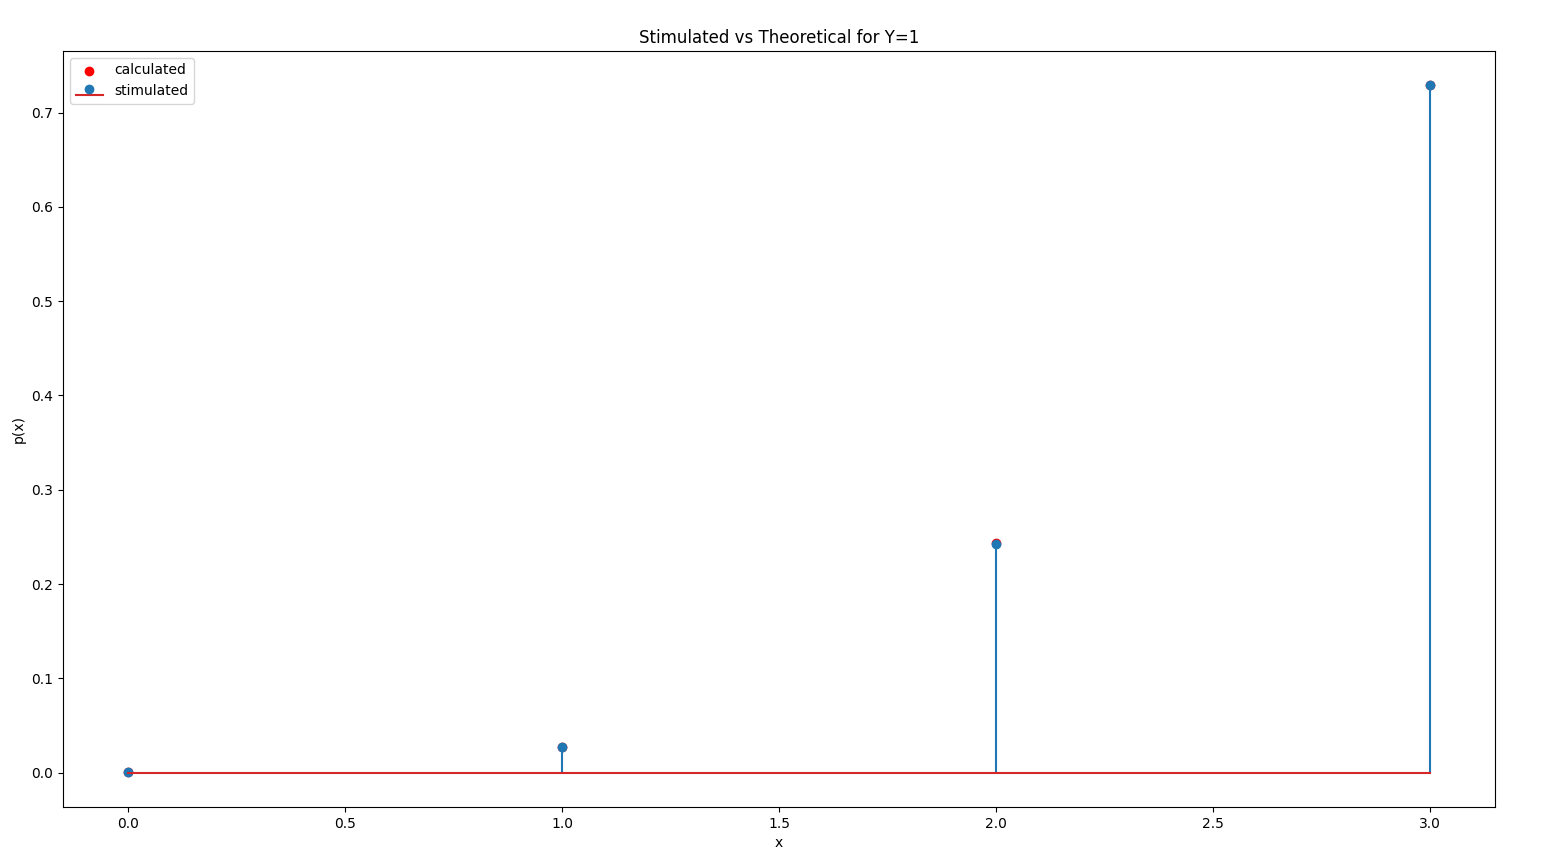
\includegraphics[width=8cm]{assignment2_plot2}
    \caption{Plot when Y = 1}
    \label{fig:2}
\end{figure}
\end{document}
